\documentclass[12pt, a4paper]{article} %determina o tamanho da fonte, o tipo de papel e o tipo de documento.

\setlength{\parindent}{1.0 cm} %tamanho do espaço para começar o parágrafo.
\setlength{\parskip}{0.5cm} %tamanho do espaço entre os parágrafos.

%Aqui ficam os pacotes utilizados para formatação do documento de modo geral:

\usepackage[utf8]{inputenc} 
\usepackage{indentfirst} %Coloca espaços nos inícios de parágrafos automaticamente. 
\usepackage[brazilian]{babel} %
\usepackage{amsmath}
\usepackage[hmargin=3cm, vmargin=2.5cm, bmargin=2.5cm]{geometry}
\usepackage{multicol}
\usepackage{graphicx} %para poder inserir imagens
\usepackage{subfig}
\usepackage{booktabs} 
\usepackage{hyperref} %para poder adicionar links e hiperlinks
\usepackage{float} %para poder posicionar as imagens


\usepackage{listings} %para poder incluir códigos
\usepackage{xcolor}
\definecolor{codegreen}{rgb}{0,0.6,0}
\definecolor{codegray}{rgb}{0.5,0.5,0.5}
\definecolor{codepurple}{rgb}{0.58,0,0.82}
\definecolor{backcolour}{rgb}{0.95,0.95,0.92}
\lstdefinestyle{mystyle}{
    backgroundcolor=\color{backcolour},   
    commentstyle=\color{codegreen},
    keywordstyle=\color{magenta},
    numberstyle=\tiny\color{codegray},
    stringstyle=\color{codepurple},
    basicstyle=\ttfamily\footnotesize,
    breakatwhitespace=false,         
    breaklines=true,                 
    captionpos=b,                    
    keepspaces=true,                 
    numbers=left,                    
    numbersep=5pt,                  
    showspaces=false,                
    showstringspaces=false,
    showtabs=false,                  
    tabsize=2,
    morecomment={l}[!],
    language=[77]Fortran,
}
\lstset{style=mystyle}

\begin{document} %começa alguma coisa,neste caso, o documento, sempre importante lembrar de colocar o \end{} para não dar erro 
	
	\begin{titlepage}
		\begin{center}
\Huge{Universidade de São Paulo}\\
\large{Instituto de Física de São Carlos}\\
\vspace{20pt}
\vspace{200pt}
\textbf{Lista 1}\\
\vspace{8cm}
		\end{center}

\begin{flushleft}
\begin{tabbing}
Pedro Calligaris Delbem 5255417\\
\end{tabbing}
\vspace{0.5cm}
Professor: Attilio Cucchieri\\		
		\end{flushleft}
	
		\begin{center}
			\vspace{\fill}
	Março de 2025	
		\end{center}
	\end{titlepage}

%####################################################################### SUMÁRIO
	\tableofcontents 
	\thispagestyle{empty}
	\newpage
%#########################################################################
\section{Exerc\'icio 1}

    Tarefa: Calcular a \'area de um c\'irculo. Op\c{c}\~oes: entrada e sa\'ida usando teclado e monitor; entrada e sa\'ida usando arquivos; calcular a  \'area em uma subrotina.

    C\'odigo Escrito:
    \lstinputlisting[language=Fortran]{../L1-5255417-ex-1.f90}

    O c\'odigo foi compilado com o comando:
    \begin{verbatim}
        gfortran L1-5255417-ex-1.f90 -o L1-5255417-ex-1.exe
    \end{verbatim}

    Resultados:
    \begin{figure}[H]
        \centering
        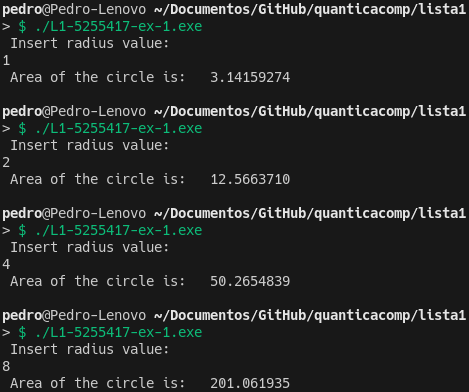
\includegraphics[width=0.8\textwidth]{../images/results-ex1.png}
        \caption{Valores de \'area para os raio de 1, 2, 4 e 8.}
    \end{figure}

    A \'area para o raio = 1 correponde ao valor de $\pi$, de acordo com o esperado. Dobrando o valor do raio espera-se, então, que o valor da \'area quadruplique e isto foi o que se obteve.

\section{Exerc\'icio 2}

    Tarefa: Testar overflow e underflow em precis\~ao simples e dupla.

    C\'odigo Escrito:
    \lstinputlisting[language=Fortran]{../L1-5255417-ex-2.f90}

    O c\'odigo foi compilado com o comando:
    \begin{verbatim}
        gfortran L1-5255417-ex-2.f90 -o L1-5255417-ex-2.exe
    \end{verbatim}

    Resultados:
    \begin{figure}[H]
        \centering
        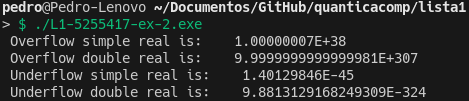
\includegraphics[width=0.8\textwidth]{../images/results-ex2.png}
        \caption{Valores de overflow e underflow para precis\~ao simples e dupla.}
    \end{figure}

    Nota-se que os valores obtidos s\~ao coerentes com o esperado.

\section{Exerc\'icio 3}

    Tarefa: Achar a precis\~ao  do computador, i.e., o maior n\'umero positivo  tal que
    1 + $\epsilon$ = 1, usando precis\~ao simples e dupla.

    C\'odigo Escrito:
    \lstinputlisting[language=Fortran]{../L1-5255417-ex-3.f90}

    O c\'odigo foi compilado com o comando:
    \begin{verbatim}
        gfortran L1-5255417-ex-3.f90 -o L1-5255417-ex-3.exe
    \end{verbatim}

    Resultados:
    \begin{figure}[H]
        \centering
        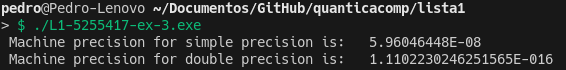
\includegraphics[width=0.8\textwidth]{../images/results-ex3.png}
        \caption{Valores de $\epsilon$ para precis\~ao para precis\~ao simples e dupla.}
    \end{figure}

    Nota-se que os valores obtidos correspondem aos valores esperados.

\section{Exerc\'icio 4}

    Tarefa: Calcular

    \begin{equation} e^{-x} = 1 - x + x^2/2! - x^3/3! + ... \end{equation}

    para x = 0.1, 1, 10, 100 e 1000 com um erro menor do que $10^{-8}$. Problema: quando truncar a s\'erie? \'E preciso calcular o fatorial explicitamente? Comparar o valor obtido usando a s\'erie com o resultado exato.

    C\'odigo Escrito:
    \lstinputlisting[language=Fortran]{../L1-5255417-ex-4.f90}

    O c\'odigo foi compilado com o comando:
    \begin{verbatim}
        gfortran L1-5255417-ex-4.f90 -o L1-5255417-ex-4.exe
    \end{verbatim}

    Resultados:
    \begin{figure}[H]
        \centering
        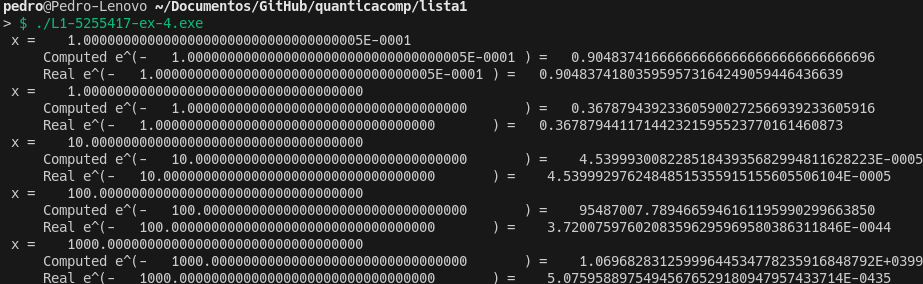
\includegraphics[width=0.8\textwidth]{../images/results-ex4.png}
        \caption{Valores de $e^{-x}$ para x = 0.1, 1, 10, 100 e 1000.}
    \end{figure}

    Por fim, percebe-se que o resultado esperado foi obtido para x = 0.1, 1 e 10. Para x = 100 e 1000 o resultado obtido diverge do esperado, o que se deve ao fato de que os termos somados se tornam muito pequenos ao ponto de serem menores que o Machine Precision.

\section{Exerc\'icio 5}

    Tarefa: Considerar a somat\'oria

    \begin{equation} \Sigma (N) = \sum_{n=1}^{2N} (-1)^n\frac{n}{n+1} = - \sum_{n=1}^N \frac{2n-1}{2n} + \sum_{n=1}^N \frac{2n}{2n+1} = \sum_{n=1}^N \frac{1}{2n(2n+1)} \end{equation}

    e calcular $\Sigma (N)$ para N = 1, 2, . . . , $10^6$ usando as tr\^es f\'ormulas acima. Comparar os resultados usando precis \~ao simples.

    C\'odigo Escrito:
    \lstinputlisting[language=Fortran]{../L1-5255417-ex-5.f90}

    O c\'odigo foi compilado com o comando:
    \begin{verbatim}
        gfortran L1-5255417-ex-5.f90 -o L1-5255417-ex-5.exe
    \end{verbatim}

    Resultados:
    \begin{figure}[H]
        \centering
        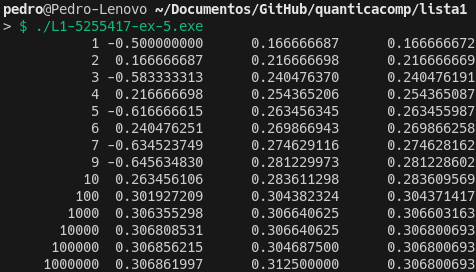
\includegraphics[width=0.8\textwidth]{../images/results-ex5.png}
        \caption{Valores de $\Sigma (N)$ para N = 1, 2, . . . , $10^6$ usando precis\~ao simples.}
    \end{figure}

    Nota-se que a primeira s\'erie demora \'e mais inst\'avel do que as demais. Al\'em disso, a terceira s\'erie se mostra mais est\'avel que a segunda - sendo ent\~ao a melhor vers\~ao.

\section{Exerc\'icio 6}

    Tarefa: Estudar numericamente o erro da aproxima\c{c}\~ao

    \begin{equation} e^{-x} \approx \sum_{n=0}^N \frac{(-x)^n}{n!} \end{equation}

    em fun\c{c}\~ao de N, para diferentes valores de x. Sugest\~ao: fa\c{c}a um gr\'afico do erro em fun\c{c}\~ao de N. O que acontece quando $e^{-x}$  \'e calculado usando a s\'erie $e^x = \sum_{n=0}^{N} \frac{x^n}{n!}$ e, depois, calculando 1/$e^x$?

    C\'odigo Escrito:
    \lstinputlisting[language=Fortran]{../L1-5255417-ex-6.f90}

    O c\'odigo foi compilado com o comando:
    \begin{verbatim}
        gfortran L1-5255417-ex-6.f90 -o L1-5255417-ex-6.exe
    \end{verbatim}

    Resultados:
    \begin{figure}[H]
        \centering
        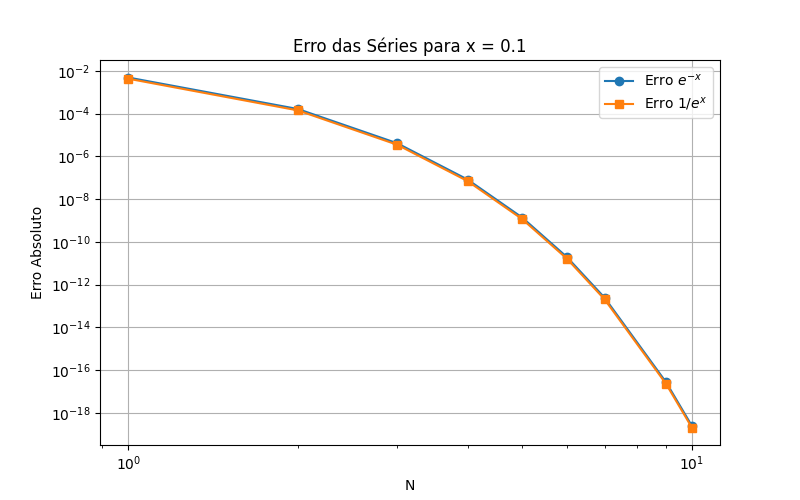
\includegraphics[width=0.8\textwidth]{../images/erro_x_0_1.png}
        \caption{Gr\'afico do erro em fun\c{c}\~ao de N para x = 0.100000001.}
    \end{figure}

    \begin{figure}[H]
        \centering
        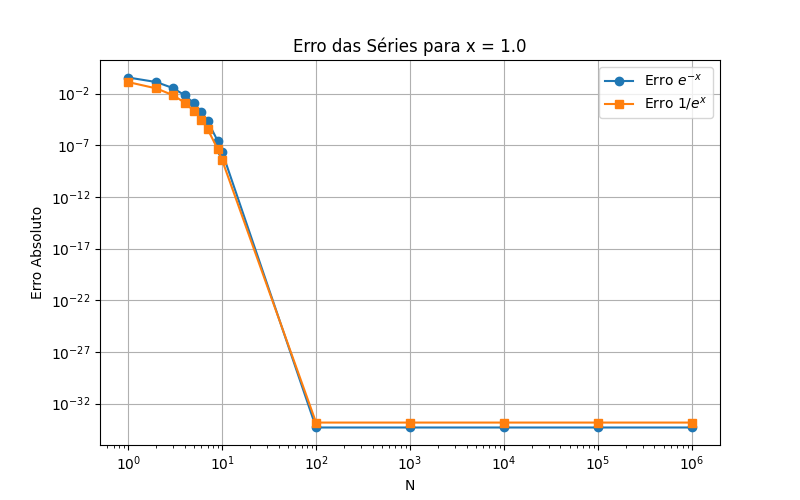
\includegraphics[width=0.8\textwidth]{../images/erro_x_1_0.png}
        \caption{Gr\'afico do erro em fun\c{c}\~ao de N para x = 1.}
    \end{figure}

    \begin{figure}[H]
        \centering
        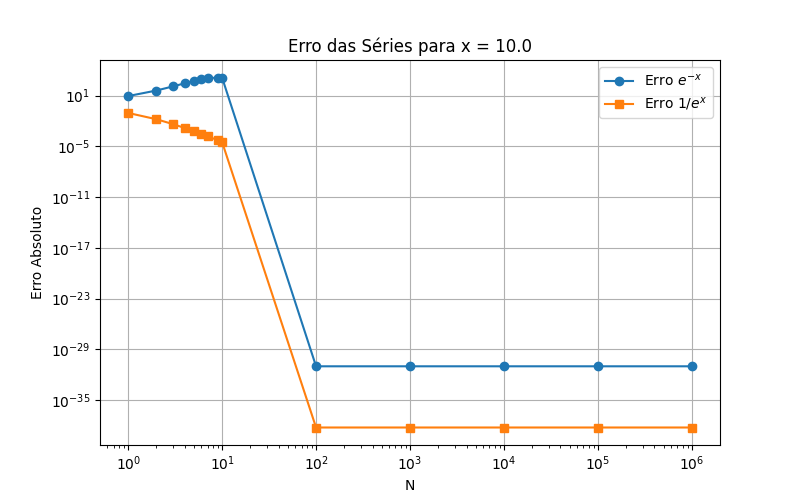
\includegraphics[width=0.8\textwidth]{../images/erro_x_10_0.png}
        \caption{Gr\'afico do erro em fun\c{c}\~ao de N para x = 10.}
    \end{figure}

    \begin{figure}[H]
        \centering
        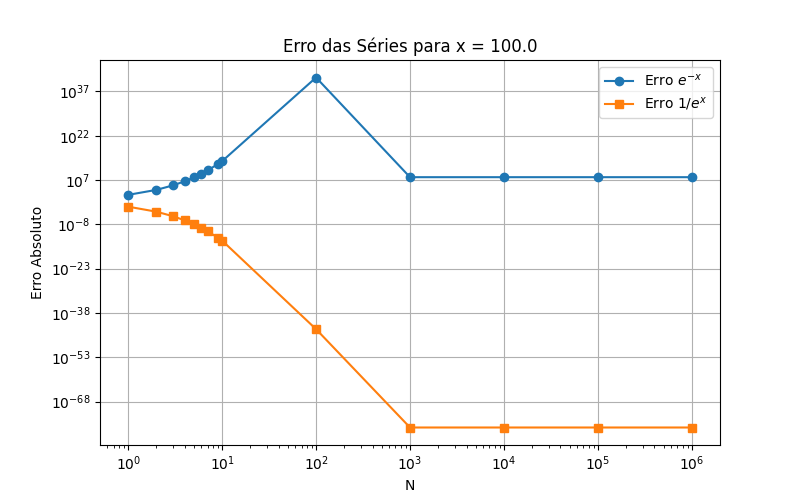
\includegraphics[width=0.8\textwidth]{../images/erro_x_100_0.png}
        \caption{Gr\'afico do erro em fun\c{c}\~ao de N para x = 100.}
    \end{figure}

    \begin{figure}[H]
        \centering
        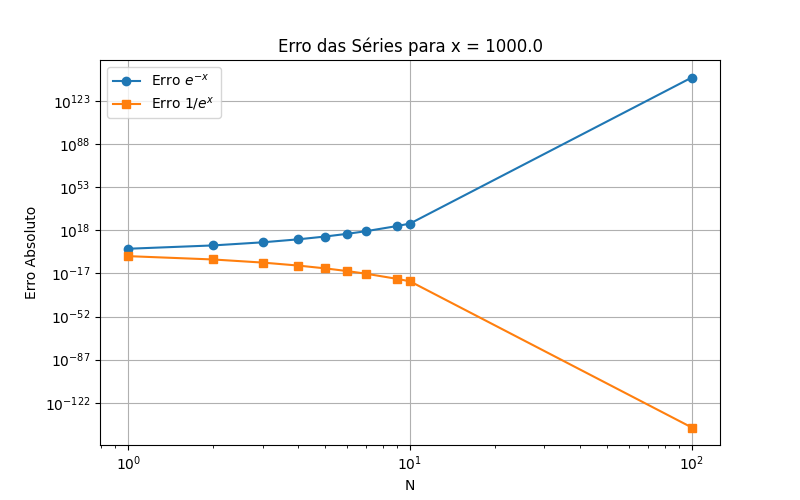
\includegraphics[width=0.8\textwidth]{../images/erro_x_1000_0.png}
        \caption{Gr\'afico do erro em fun\c{c}\~ao de N para x = 1000.}
    \end{figure}

    Percebe-se - claramente - que calcular a s\'erie de $e^x$ e fazer 1/$e^x$ o resultado \'e mais preciso do que calcular a s\'erie, diretamente, de $e^{-x}$. Al\'em disso, \'e not\'orio que ao calcular a s\'erie de $e^{-x}$  diretamente para valores de N muito grande o resultado apresenta uma diverg\^encia muito grande do resultado real o que se deve ao fato de que os termos somados se tornam muito pequenos ao ponto de serem menores que o Machine Precision.

\end{document}